\chapter[Learning Conditional Random Fields]{Learning\linebreak[4] Conditional Random Fields}\label{ch:structured_pystruct}

Many classical computer vision applications such as stereo, optical flow, semantic
segmentation and visual grouping can be naturally formulated as image labeling tasks.
%
Arguably the most popular way to approach such labeling problems is via graphical
models, such as Markov random fields (MRFs) and conditional random fields (CRFs).
MRFs and CRFs provide a principled way of integrating local evidence and
modeling spatial dependencies, which are strong in most image-based tasks.
%
While in earlier approaches, model parameters were set by hand or using
cross-validation, more recently parameters are often learned using a max-margin
approach.

Most models employ linear energy functions of unary and pairwise interactions,
trained using structural support vector machines (SSVMs). While linear energy
functions lead to learning problems that are convex in the parameters, complex
constraints complicate their optimization.  % computation? ;)

In recent years there has been a wealth of research in methods for learning
structured prediction, as well as in their application in areas such as natural
language processing and computer vision (see \citet{nowozin2011structured}
for an introduction and \citet{blake2011markov} for a recent survey).
%
In this chapter, we first introduce the concepts and algorithms used in
structured prediction, in particular in maximum margin methods. We 
accompany this by a description of our open source implementation of these
algorithms, \pystruct.

\pagebreak

\section{Basic Concepts in Structured Prediction}\seclabel{basics_structured_prediction}

Structured prediction can be defined as making a prediction $f(x)$ by
maximizing a compatibility function $g$ between an input $x$ and possible
labels
$y$~\citep{nowozin2011structured}:
\begin{equation}
    f(x) = \argmax_{y \in \mathcal{Y}} g(x, y)
\end{equation}
Finding $y$ in the above equation is often referred to as inference
or prediction.
Most current approaches use linear functions, with some notable exceptions:
\citet{peng2009conditional} introduced a conditional random field for sequence
prediction where single-node potentials are computed using neural networks,
while \citet{nowozin2011decision} proposed a conditional random field for image
processing, where all potentials are computed using decision trees.

The linear approach leads to
\begin{equation}\eqlabel{main_equation}
    f(x) = \argmax_{y \in \mathcal{Y}}\  \theta^T \Phi(x, y).
\end{equation}
Here, $y$ is a \emph{structured} label, $\Phi$ is a joint feature function of
$x$ and $y$, and $\theta$ contains the parameters of the model. \emph{Structured} means
that $y$ is more complicated than a single output class, for example a label
for each word in a sentence or a label for each pixel in an image.
Learning structured prediction means learning the parameters $\theta$ from
training data.  The particular model that is used is completely encoded in
$\Phi(x, y)$, which manifests the relation between input $x$ and output $y$. As
$\mathcal{Y}$ is typically very large, it is crucial to exploit the particular
form of $\Phi(x, y)$ to solve the prediction problem of \Eqref{main_equation}.

While $y$ could be complicated like a parse tree or the geometric
configuration of a molecule, many settings, such as the image segmentation
setting we are interested in, can be reduced to the case where $y$ is a vector of
discrete labels $\mathcal{Y} = \{1, \dotsc, k\}^n$.
In the following, we only discuss this multivariate case. In general, $n$
is often different for different inputs $x$, such as images with different
numbers of pixels.  We ignore this in our notation to simplify the
presentation.

\subsection{Factor Graphs and the Relation to Graphical Models}\seclabel{factor_graphs}
% one factor graph per instance? FIXME
In the case when $y$ is multivariate, a very general and widely used method to
specify the structure of a model, and therefore $\Phi$, is using \emph{factor
graphs}. A factor graph is a bipartite graph $(\mathcal{V}, \mathcal{F},
\mathcal{E})$, consisting of variable nodes $\mathcal{V}$, factor nodes
$\mathcal{F}$ and edges $\mathcal{E}$ connecting variables to factors. The
\emph{scope} $N_F$ of a factor $F \in \mathcal{F}$ is defined as
\begin{equation}
    N_F = \{ v \in \mathcal{V} \,|\, (v,F) \in \mathcal{E} \}
\end{equation}
The variable nodes of the factor graph correspond to the entries of the
variables $y$, that is $\mathcal{V} = \{1, \dotsc, n\}$, and each factor node
is associated with a \emph{factor} or \emph{potential function} $\psi_F$.
A factor graph represents a function\footnote{Traditionally factor graphs
 represent \emph{products} of factors.  To simplify presentation, we work
directly in the log-domain of the more standard product representation.}
\begin{equation}\eqlabel{log_factor_graph}
    g(x, y) = \sum_{F \in \mathcal{F}} \psi_F(x, y_{N_F})
\end{equation}
Here, $y_{N_F}$ denotes the entries of $y$ indexed by $N_F$.

The benefit of using the factor graph representation is that it decomposes the
function over subsets of the variables of interest $y_i$. This allows us to apply
efficient optimization procedures for the prediction problem in
\Eqref{main_equation} by exploiting the graph structure of the factor graph.
%
To obtain a linear function from
\Eqref{log_factor_graph} as in \Eqref{main_equation}, we can simply let each $\psi$ be of the form
\begin{equation}\eqlabel{general_psi}
    \psi_F(x, y_{N_F}) = \theta_F^T \Phi_F(x, y_{N_F}).
\end{equation}
The most common form by far is 
\begin{equation}\eqlabel{linear_psi}
    \psi_F(x, y_{N_F}) = \theta_{F, y_{N_F}}^T \phi_F(x),
\end{equation}
where $\phi_F(x)$ is a vector representation of the input $x$, and there are
different parameter vectors $\theta_{F, y_{N_F}}$ for each possible assignment
of $y_{N_F} \in \mathcal{Y}_{N_F}$.
%
Both, \Eqref{general_psi} and \Eqref{linear_psi} are instantiations of the general
linear form \Eqref{main_equation}. To see this, for \Eqref{general_psi} we simply
concatenate the individual components for all $f \in \mathcal{F}$:
\begin{align}
    \theta &= \bigoplus_{F \in \mathcal{F}} \theta_F\\
    \Phi(x, y) &= \bigoplus_{F \in \mathcal{F}} \Phi_F(x, y_{N_F}).
\end{align}
Writing down $\Phi$ and $\theta$ for the form \Eqref{linear_psi} is a little less compact:
\begin{align}
    \theta &= \bigoplus_{F \in \mathcal{F}}\ \bigoplus_{y_{N_F} \in \mathcal{Y}_{N_F}} \theta_{F, y_{N_F}}\\
    \Phi(x, y) &= \bigoplus_{F \in \mathcal{F}} \left (\phi_F(x) \otimes e_{y_{N_F}} \right ),
\end{align}
Here $e_{y_{N_F}} \in \mathbb{R}^{|\mathcal{Y}_{N_F}|}$ is the indicator for a
given variable setting $y_{N_F}$.
In words, $\Phi_F$ is built simply by creating a vector of
$|\mathcal{Y}_{N_F}|$ times the size of $\phi_F$, which is zero everywhere,
except for the position corresponding to $y_{N_F}$. %TODO unclear!

This approach to structured prediction is closely related to 
approaches using \emph{probabilistic graphical models}.  Probabilistic graphical models are a
tool to express factorizations of probability distributions.  Similar to
\Eqref{log_factor_graph}, the joint probability distribution over a
multi-variate random variable $y$ can be expressed using a factor-graph:
\begin{equation}\eqlabel{graphicalmodel}
    p(y | x) = \frac{1}{Z_x}\prod_{F \in \mathcal{F}} \exp\left(\psi_F(x, y_{N_F})\right).
\end{equation}
Here
\begin{equation}
    Z_x = \sum_{y' \in \mathcal{Y}} \prod_{F \in \mathcal{F}} \exp\left(\psi(x, y'_{N_F})\right)
\end{equation}
is the normalization constant of the conditional distribution over $y$.
If $f$ is chosen as in \Eqref{linear_psi}, then the resulting distribution
belongs to the exponential family, the class of probability distributions most
commonly used in the graphical model literature.

The most probable prediction $y$ is given as $\displaystyle \argmax_{y \in \mathcal{Y}}p(y|x)$.
As $Z$ is independent of $y$, and by the monotonicity of the logarithm,
maximizing $p(y|x)$ is equivalent to maximizing $g(x,y)$ over $y$ in
\Eqref{log_factor_graph}. Therefore, from a prediction standpoint, the two
formulations are equivalent.

During learning, the presence of the factor $Z$ in \Eqref{graphicalmodel}
introduces additional complications. As we only address the problem of making
predictions, not modeling probabilities, there are no clear benefits from the
probabilistic approach.  Consequently, we work with the more direct
structured prediction approach of \Eqref{main_equation} and
\Eqref{log_factor_graph} instead.


\section{Learning Max-Margin Structured Prediction}\seclabel{learning_algorithms}

Maximum margin learning has become one of the most popular methods to learn
classifiers and structural models in computer vision and text processing.
There are several reasons for the popularity of linear maximum margin approaches:
\begin{description}
    \item[Loss-sensitivity] In contrast to most probabilistic approaches, maximum margin learning approaches can directly
        minimize a user-specified loss.
    \item[Feasibility] If the loss decomposes over the factor graph that
        specifies $g$, then learning is feasible as soon as the maximization
        over $y$ in \Eqref{main_equation} can be carried out.
    \item[Generalization] The maximum margin principle yields generalization
        bounds using the effective complexity~\citep{taskar2003max}, that are generally
        tighter than corresponding VC-theoretical bounds.
    \item[Strong Convexity] The resulting optimization problem is strongly
        convex, leading to efficient optimization and unique solutions.
\end{description}

For learning, a dataset $(x\hoch{1}, y\hoch{1}),\dotsc,(x\hoch{k}, y\hoch{k})$ is given, together with a loss
\begin{equation}
    \Delta \colon \mathcal{Y} \times \mathcal{Y} \rightarrow \mathbb{R}.
\end{equation}
The parameters $\theta$ are learned by minimizing the loss-based soft-margin
objective
\begin{equation}\eqlabel{learning_equation}
    \min_\theta \frac{1}{2} ||\theta||^2 + C \sum_i  \ell(x\hoch{i}, y\hoch{i}, \theta)
\end{equation}
with regularization parameter $C$.\pagebreak\\
Here, $\ell$ is a hinge-loss-like upper bound
on the empirical $\Delta$-risk:
\begin{equation}\eqlabel{loss_augmentation}
    \ell(x\hoch{i}, y\hoch{i}, \theta) = [\max_{y \in \mathcal{Y}} \Delta(y\hoch{i}, y) + \theta^T \Phi(x\hoch{i}, y) - \theta^T \Phi(x\hoch{i}, y\hoch{i})]_+.
\end{equation}
This is an instance of regularized empirical risk minimization, with a
piecewise linear, convex upper bound on the loss. 
Finding the $y$ that corresponds to a maximum in \Eqref{loss_augmentation} is
a central part of all maximum-margin based learning algorithms, and is referred to
as loss-augmented prediction. For complex models, such as the ones used for
image segmentation, this optimization often dominates the learning process in
terms of computational complexity.
Therefore, it is often desirable to find learning algorithms that converge with
as little optimizations of the loss-augmented prediction problem as possible.

There are several popular algorithms to solve \Eqref{learning_equation}. We
briefly review three standard algorithms, and a very recent one: the
$1$-slack and $n$-slack cutting plane algorithms, a stochastic primal subgradient
algorithm, and recently proposed stochastic dual coordinate descent method,
which we now describe in detail. We also give simplified known
convergence rates in terms of calls to the loss-augmented prediction.

Additionally, we discuss practical implications and implementation.  One
particularly interesting aspect is the difference between \emph{sequential}
(or \emph{online}) and \emph{batch} algorithms.  Batch algorithms process the
whole dataset before adjusting parameters, while sequential algorithms process
one sample at a time, and adjust parameters incrementally.
In image segmentation tasks, inference is often costly, making loss-augmented
prediction the most expensive step in learning. This often leads to longer
run-times for batch algorithms. On the other hand, loss-augmented prediction in
batch algorithms is \emph{embarrassingly parallel}, allowing the use of multiple
processors with almost linear speed improvements.

\subsection{Stochastic Subgradient Descent}\seclabel{subgradient}

Arguably the most straight-forward way to approach \Eqref{learning_equation} is
using subgradient descent.  In light of the complexity of solving the
loss-augmented prediction problem in \Eqref{loss_augmentation}, it is natural
to work in a stochastic setting (see \citet{ratliff2007online}).\pagebreak\\
Given a model through $\Phi$ and a set of parameters $\theta$, a subgradient
considering a single training example $(x\hoch{i}, y\hoch{i})$
can be computed simply by solving the loss-augmented prediction problem:
\begin{align*}
    &\frac{d}{d\theta} \left [ \frac{1}{2} ||\theta||^2 + C \ell(x\hoch{i}, y\hoch{i}, \theta) \right ] \ni C\left [ \Phi(x\hoch{i}, \hat{y}) - \Phi(x\hoch{i}, y\hoch{i}) \right]+ \theta\numberthis\\
    &\text{with }\hat{y} \in \argmax_{y \in \mathcal{Y}} \Delta(y\hoch{i}, y) + \theta^T \Phi(x\hoch{i}, y)
\end{align*}
The most commonly used update has the simple form
\begin{equation}
    \theta_{t+1} = (1 - \eta_t) \theta_t - \eta_t C \left [\Phi(x\hoch{i}, \hat{y}) - \Phi(x\hoch{i}, y\hoch{i})\right]
\end{equation}
Where $\eta_t$ is a sequence of step sizes.
%Theoretical convergence guarantees of \ldots can be given whenever \ldots,
In practice the choice of $\eta_t$ is often strongly influences the convergence behavior.
Many practitioners adopt the sequence proposed for binary SVMs in the Pegasos algorithm~\citep{shalev2011pegasos}:
\begin{equation}
    \eta_t = \frac{C}{t},
\end{equation}
which has been found to work well in many settings.
\citet{shalev2011pegasos} showed that this schedule achieves a convergence rate of $O(\frac{\ln T }{T})$.
\citet{lacoste2012block} and \citet{shamir2012stochastic} recently showed independently that
a rate of $O(\frac{1}{T})$ can be achieved using a novel averaging scheme:
\begin{equation}
    \bar{\theta}_{T} = \frac{2}{(T+1)(T+2)} \sum_{t=0}^T(t+1) \theta_t.
\end{equation}
This $t$-weighted averaging can be computed on-the-fly as
\begin{equation}\eqlabel{averaging}
    \bar{\theta}_{t} = \frac{t}{t + 2} \bar{\theta}_t + \frac{2}{t+2} \theta_{t+1}.
\end{equation}

Implementation of the stochastic subgradient algorithm (with or without
averaging) is straight-forward, but unfortunately detecting convergence is
often tricky.
It is possible to use mini-batches instead of processing one sample at a time
to make use of multiple processors for loss-augmented prediction. Unfortunately,
this negatively affects the number of iterations needed, and did not provide a
benefit in our experiments.

\begin{algorithm*}[t]
    \caption{$n$-Slack Cutting Plane Training of Structural SVMs \label{alg_n_slack}}
    \begin{doublespacing}
    \begin{algorithmic}[1]
        \Require training samples $\{ (x\hoch{1}, y\hoch{1}), \dots, (x\hoch{k}, y\hoch{k})\}$, regularization parameter $C$, stopping tolerance $\epsilon$.
        \Ensure parameters $\theta$, slack $(\xi_1, \dotsc, \xi_k)$
        \State $\W_i \leftarrow \varnothing, \xi_i \leftarrow 0 \text{ for } i=1,\dots,k$
        \Repeat
            \For {i=1, \dots, k}
                \State
                $\hat{y} \leftarrow I(x\hoch{i}, y\hoch{i}, \theta) := \displaystyle \argmax_{\hat{y}\in\mathcal{Y}} \delta(y\hoch{i}, \hat{y}) - \theta^T [\Phi(x\hoch{i}, y\hoch{i}) - \Phi(x\hoch{i}, \hat{y})] $
                \If{$\displaystyle \delta(y\hoch{i}, \hat{y}) - \theta^T [\Phi(x\hoch{i}, y\hoch{i}) - \Phi(x\hoch{i}, \hat{y})] \geq \xi_i + \epsilon$}
                \State \hspace{-3mm}$\W_i \leftarrow \W_i \cup \{ \hat{y}\} $
                    \State
                    \vspace{-15mm}
                    \begin{flalign*}
                        \qquad\qquad(\theta, \xi_1, \dots, \xi_k) \leftarrow \displaystyle \argmin_{\theta, \xi_1, \dots, \xi_k}& \frac{||\theta||}{2}^2 + C \sum_{i=1}^k\xi_i&\\
                        \text{s.t. }& \text{for } i=1,\dots,k\ \forall \hat{y} \in \W_i:&\\
                                    &\theta^T [\Phi(x\hoch{i}, y\hoch{i}) - \Phi(x\hoch{i}, \hat{y}\hoch{i})] \geq \delta(y\hoch{i}, \hat{y}\hoch{i}) - \xi_i&
                    \end{flalign*}
                \EndIf
            \EndFor
            \vspace{-10mm}
            \Until no $\W_i$ changes anymore.
        \end{algorithmic}
    \end{doublespacing}
    \end{algorithm*}

\subsection{The $n$-Slack Cutting Plane Method}\seclabel{n_slack}

The $n$-slack cutting plane method~\citep{tsochantaridis2006large} reformulates \Eqref{learning_equation}
into a quadratic objective with a combinatorial number of constraints:
\begin{align*}
    \min_{\theta, \xi_1, \dots, \xi_k}\ &\frac{1}{2} ||\theta||^2 + C \sum_{i=1}^k \xi_i \numberthis \label{eq:nslack}\\
    \text{s.t. }&\text{for } i=1,\dots,k\ \forall \hat{y} \in \mathcal{Y}:\\
    &\theta^T [\Phi(x\hoch{i}, y\hoch{i}) - \Phi(x\hoch{i},
        \hat{y})] \geq \Delta(y\hoch{i}, \hat{y})
            - \xi_i
\end{align*}
As it is not feasible to deal with all constraints, only a working set $\W$ of active constraints
is maintained, using the cutting plane method. The algorithm starts with an empty working set,
and repeatedly iterates over the training data. For each sample, the most
violated constraint is added to $\W$, and the quadratic program is solved
again, with the new set of constraints.
The algorithm terminates when no constraint can be found that is violated more than $\epsilon$,
which guarantees a suboptimality of at most $\epsilon$.
%
\citet{tsochantaridis2006large} showed a convergence rate of $O(\frac{1}{T^2})$
with respect to calls to the QP solver. In the worst-case, only a single new constraint
could be found in one pass over the dataset, which leads to $O(\frac{1}{kT^2})$ in terms
of calls to loss-augmented prediction. The recent work
of~\citet{lacoste2012block}, however, suggests a rate of $O(\frac{1}{T})$,
which empirically seems more plausible. This analysis does not include the cost
of solving the QP, which depends on the size of the dataset and the number of
iterations. 
The complete procedure is described in Algorithm~\ref{alg_n_slack}.

The $n$-slack cutting plane is a sequential algorithm that processes each sample
individually. While this allows fast process of the optimization with respect
to the number of calls to loss-augmented prediction, individual steps
become more and more costly. The number of the constraints is usually a
multiple of the number of training  samples, which leads to very large QP
problems, even for medium sized datasets. This makes the algorithm often slow
in practice.
%
Solving the quadratic program can be accelerated using several techniques. We
found that aggressively removing constraints that are inactive or contribute
little to the solution often makes the difference between the algorithm being
practical or not.  Another possible technique is to update the quadratic
program only every $r$ samples, for some small integer $r$
(\citet{joachims2009cutting} suggest $r=100$). While this strategy on its own did
not provide a large benefits in our experiments, it allows for parallel
loss-augmented prediction on these mini-batches of size $r$.


\subsection{The $1$-Slack Cutting Plane Method}\seclabel{one_slack}

\begin{algorithm*}[t]
    \caption{$1$-Slack Cutting Plane Training of Structural SVMs \label{alg_one_slack}}
    \begin{algorithmic}[1]
        \Require training samples $\{ (x\hoch{i}, y\hoch{i}), \dots, (x\hoch{i}, y\hoch{i})\}$, regularization parameter $C$, stopping tolerance $\epsilon$.
        \Ensure parameters $\theta$, slack $\xi$
        \State $\W \leftarrow \emptyset$
        \Repeat
            \State 
            \vspace{-5mm}
            \begin{flalign*}
                \quad\,\,(\theta, \xi) \leftarrow \displaystyle \argmin_{\theta, \xi}&\frac{||\theta||}{2}^2 + C \xi&\\
                \text{s.t. }&\forall \hat{\mathbf{y}}=(\hat{y}\hoch{1}, \dots, \hat{y}\hoch{k}) \in \W:&\\
                            &\theta^T \sum_{i=1}^k [\Phi(x\hoch{i}, y\hoch{i}) - \Phi(x\hoch{i}, \hat{y}\hoch{i})] \geq \sum_{i=1}^k \delta(y\hoch{i}, \hat{y}\hoch{i}) - \xi&
            \end{flalign*}
            \For {i=1, \dots, k}
                \State
                $\hat{y}\hoch{i} \leftarrow I(x\hoch{i}, y\hoch{i}, \theta) := \displaystyle \argmax_{\hat{y}\in\mathcal{Y}} \sum_{i=1}^k \delta(y\hoch{i}, \hat{y}) - \theta^T \sum_{i=1}^k [\Phi(x\hoch{i}, y\hoch{i}) - \Phi(x\hoch{i}, \hat{y})]$ \label{get_cutting_plane}
            \EndFor
            \State $\W \leftarrow \W \cup \{ (\hat{y}\hoch{i}, \dots, \hat{y}\hoch{i}) \} $
            \State $ \displaystyle \xi' \leftarrow  \sum_{i=1}^k \delta(y\hoch{i}, \hat{y}\hoch{i}) - \theta^T \sum_{i=1}^k [\Phi(x\hoch{i}, y\hoch{i}) - \Phi(x\hoch{i}, \hat{y}\hoch{i})] $
        \Until $\xi' - \xi < \epsilon$ \label{convergence_check}
    \end{algorithmic}
\end{algorithm*}

The $1$-slack cutting plane method~\citep{joachims2009cutting} solves the
following reformulation of Equation~\Eqref{learning_equation}:
\begin{align*}
    \min_{\theta, \xi}\ &\frac{1}{2} ||\theta||^2 + C \xi \numberthis\label{eq:oneslack}\\
    \text{s.t. }&\forall \hat{\mathbf{y}}=(\hat{y}^1, \dots, \hat{y}^n) \in \mathcal{Y}^n:\\
        &\theta^T \sum_{i=1}^n [\Phi(x^i, y^i) - \Phi(x^i,
            \hat{y}^i)] \geq \sum_{i=1}^n \Delta(y^i, \hat{y}^i)
            - \xi
\end{align*}
\enlargethispage{10mm}
Informally, the $1$-slack formulation corresponds to joining all training
samples into a single training example $(\mathbf{x}, \mathbf{y})$ that has no
interactions between variables corresponding to different data points, and
then applying the $n$-slack algorithm with a single data point.\pagebreak\\
A detailed description can be found in Algorithm~\ref{alg_one_slack}.
%
By construction, only a single constraint is added in each iteration of
Algorithm~\ref{alg_one_slack}, leading to very small working sets $\W$.
This has the advantage of producing a QP that easier to solve, as it contains far
less variables than in the $n$-slack algorithm. The down-side of this is that
the loss-augmented prediction problem has to be solved much more often until
convergence. This is reflected in a convergence rate of $O(\frac{1}{kT})$,
which scales with the inverse of the dataset size.

\citet{joachims2009cutting}, who introduced the method, proposed two enhancements
to make the algorithm more efficient:
\begin{description}
    \item[Constraint Pruning] As in the $n$-slack algorithm, members of the
        working set $\W$ can become inactive during learning.  If a constraint
        has been inactive for a number of iterations, it is removed from $\W$,
        leading to smaller problem sizes.
    \item[Inference Caching] In the $1$-slack algorithm, each constraint is
        created using a combination of loss-augmented prediction results.
        Therefore, each of these predictions can be part of multiple
        constraints during learning.
        To exploit this, we maintain a set $C^i$ of the last $r$ results of
        loss-augmented prediction for each training example $(x^i, y^i)$
        (line~\ref{get_cutting_plane} in Algorithm~\ref{alg_one_slack}).
        For generating a new constraint $(\hat{y}^1, \dotsc, \hat{y}^n)$, we
        find
        \begin{equation}
            \hat{y}^i \leftarrow \argmax_{\hat{y}\in C^i} \sum_{i=1}^n
            \Delta(y^i, \hat{y}) - \theta^T \sum_{i=1}^n [\Phi(x^i, y^i) -
                \Phi(x^i, \hat{y})] 
        \end{equation}
        by enumeration of $C^i$ and continue until
        line~\ref{convergence_check}.  Only if $\xi' - \xi < \epsilon$, that is
        the produced constraint is not violated strongly enough, we return to
        line~\ref{get_cutting_plane} and actually invoke the loss augmented
        prediction $I$.
\end{description}

\subsection{The SZLJSP Algorithm}\seclabel{dual_coordinate_descent}
\begin{algorithm}[tp]
    \caption{Shalev-Shwartz Zhang Lacoste-Julien Jaggi Schmidt Pletscher\label{alg_szljsp}}
    \begin{doublespacing}
    \begin{algorithmic}[1]
        \Require training samples $\{ (x\hoch{i}, y\hoch{i}), \dots, (x\hoch{i}, y\hoch{i})\}$, regularization parameter $C$, stopping tolerance $\epsilon$.
        \Ensure parameters $\theta$
        \State  $\displaystyle \theta_0^{\vphantom{i}}, \theta_0\hoch{i}, \bar{\theta}_0^{\vphantom{i}} \leftarrow \mathbf{0},\quad \ell_0^{\vphantom{i}}, \ell_0\hoch{i}, t \leftarrow 0 $
        \Repeat
            \State $t \leftarrow t + 1$
            \State Pick $i$ uniformly at random from $\{1, \dotsc, k\}$.
            \State Perform loss-augmented prediction on sample $i$:
            \Statex[2]   $\hat{y} \leftarrow I(x\hoch{i}, y\hoch{i}, \theta) := \displaystyle \argmax_{\hat{y}\in\mathcal{Y}} \Delta(y\hoch{i}, \hat{y}) - \theta^T [\Phi(x\hoch{i}, y\hoch{i}) - \Phi(x\hoch{i}, \hat{y})]$
            \State Compute parameter and loss updates based on sample $i$:
            \Statex[2]     $\theta_s \leftarrow \frac{C}{n} \Phi(x, \hat{y})$
            \Statex[2]     $\ell_s \leftarrow \frac{C}{n} \delta(y\hoch{i}, \hat{y})$
            \State Compute optimum step size $\eta$:
            \Statex[2]    $\eta \leftarrow \frac{(\theta_t\hoch{i} - \theta_s)^T \theta_t + C (\ell_s - \ell_k\hoch{i} )}{\lVert \theta_t\hoch{i} - \theta_s \rVert^2}$ and clip to $[0, 1]$
            \State Update per-sample parameters and loss estimate:
            \Statex[2]    $\theta_{t+1}\hoch{i} \leftarrow (1 - \eta) \theta_{t+1}\hoch{i} + \eta \theta_s$
            \Statex[2]    $\ell_{t+1}\hoch{i} \leftarrow (1 - \eta) \theta_{t+1}\hoch{i} + \eta \ell_s$
            \State Update global parameters and loss estimate:
            \Statex[2]   $\theta_{t+1} \leftarrow \theta_{t+1} + \theta_{t}\hoch{i} - \theta_{t+1}\hoch{i}$
            \Statex[2]   $\ell_{t+1} \leftarrow \ell_{t+1} + \ell_{t}\hoch{i} - \ell_{t+1}\hoch{i}$
            \State Compute the weighted running average:
            \Statex[2] $\bar{\theta}_{t+1} = \frac{k}{k + 2} \bar{\theta}_k + \frac{2}{k + 2}\theta_{k+1}$
        \Until $(\theta - \theta_s)^T\theta - \ell + \ell_s \leq \epsilon$
        \Statex where $\theta_s$ and $\ell_s$ are recomputed over the whole dataset.
    \end{algorithmic}
    \end{doublespacing}
\end{algorithm}

Very recently, two groups independently derived a very performant new algorithm.
\citet{shalev2012proximal} investigated stochastic dual coordinate descent applied
to structured support vector machines. \citet{lacoste2012block} started from the Frank-Wolfe algorithm %TODO details
and derived a block-coordinate version, where each block corresponds to the
constraints associated with a single training example.  Both groups showed that
closed-form line search is possible, and, surprisingly ended up with the exact
same algorithm and closely related convergence guarantees.  The algorithm
processes a single training example at a time, and can be applied while
remaining completely in the primal domain, making it applicable to very large
datasets.  We refer to the algorithm as SZLJSP, after the authors of the
two papers.
%
The SZLJSP algorithm has the same theoretical convergence rate of $O(\frac{1}{T})$
as stochastic subgradient decent, but has two distinguishing advantages:
\begin{description}
\item[Stopping Criterion] Both views of SZLJSP give rise to a dual objective,
    which can be used as a theoretically sound stopping criterion.
\item[Learning Rate] While there are several theoretical results on choosing
    the step size in stochastic subgradient descent, choosing a concrete
    schedule is often problematic in practice. By using analytic line-search,
    SZLJSP removes the need for any step size parameter, making application
    of the algorithm much simpler.
\end{description}

In practice, the SZLJSP algorithm is usually used with the weighted averaging
described in \Eqref{averaging}, as this is known to improve performance in the
closely related stochastic subgradient algorithms, and empirically improves
convergence.
\enlargethispage{10mm}
The detailed procedure as given by \citet{lacoste2012block} is shown in Algorithm~\ref{alg_szljsp}.


\section{Conditional Random Fields for Semantic Segmentation}\seclabel{semantic_segmentation}
%
\subsection{Fundamentals of Conditional Random Fields}
Structured models based on factor graphs, as described in \Secref{factor_graphs} are often
referred to as Conditional Random Fields (CRFs), pointing to their
probabilistic interpretation.
CRFs have been established as an important tool in many areas of computer
vision. Applications include dense stereo, optical flow, inpainting,
denoising, image editing, low-level segmentation and semantic segmentation.

Most conditional random fields only apply unary and pairwise potential
functions. In this case, \Eqref{log_factor_graph} becomes
\begin{equation}\eqlabel{energy_crf}
    g(x, y) = \sum_{v \in V} \psi_v(x, y_v) + \sum_{(v, w) \in E} \psi_{v,w}(x, y_{v}, y_{w}).
\end{equation}
Here $V$ enumerates variables and $E\subset V \times V$ is a set of edges which
represent pairwise factors.

There are broadly two types of models that are used: models in which each pixel
in an image is represented as a variable, and models in which pixels are first
grouped together into superpixels and each superpixel is represented as a
variable.  In pixel-based CRFs edges are usually introduced between adjacent
pixels, that is using either 4-neighborhoods or 8-neighborhoods.
Superpixel-based approaches introduce edges between adjacent superpixels, that
is those that share a boundary. \Figref{superpixel_illustration} shows a
sample image together with extracted superpixels and the neighborhood graph.

By nature, models over pixels and models over superpixels create graphs with a
large number of loops. This complicates prediction and learning, and is the
central topic of Chapter~\ref{ch:exact_learning}.

The motivation for using superpixels is that it is often easy to group nearby
pixels that belong to the same object just based on local color or texture cues.
While it is hard to even define what makes a sensible segmentation of an image,
it is much easier to define an \emph{over-segmentation}.
The only requirement for an over-segmentation is that each segment only
contains pixels belonging to the same entity.

Using superpixels instead of pixels has large computational advantages.  A
model that uses superpixels contains much fewer variables than one that works
on pixel-level. Typical sizes for superpixels are in the hundreds of pixels,
leading to a hundred-fold decrease in the number of variables. There are also
semantic advantages. Using superpixels can constitute a form of regularization,
including prior knowledge about the structure of images. Modeling interactions
between superpixels also allows more distant parts of an image to interact,
instead of modeling long-term relations only indirectly over neighbors.
Finally, modeling decisions on a superpixel-level allows for more context for a
local decision, while semantic decisions on pixel-level are not meaningful near
object boundaries.  The main disadvantage of superpixel-based approaches is
that the initial over-segmentation can not be influenced by later reasoning.
This can be a problem if fine structures need to be segmented for which local
evidence does not suffice.
%
\begin{figure}
    \begin{tabu} to \linewidth{@{}XX@{}}
    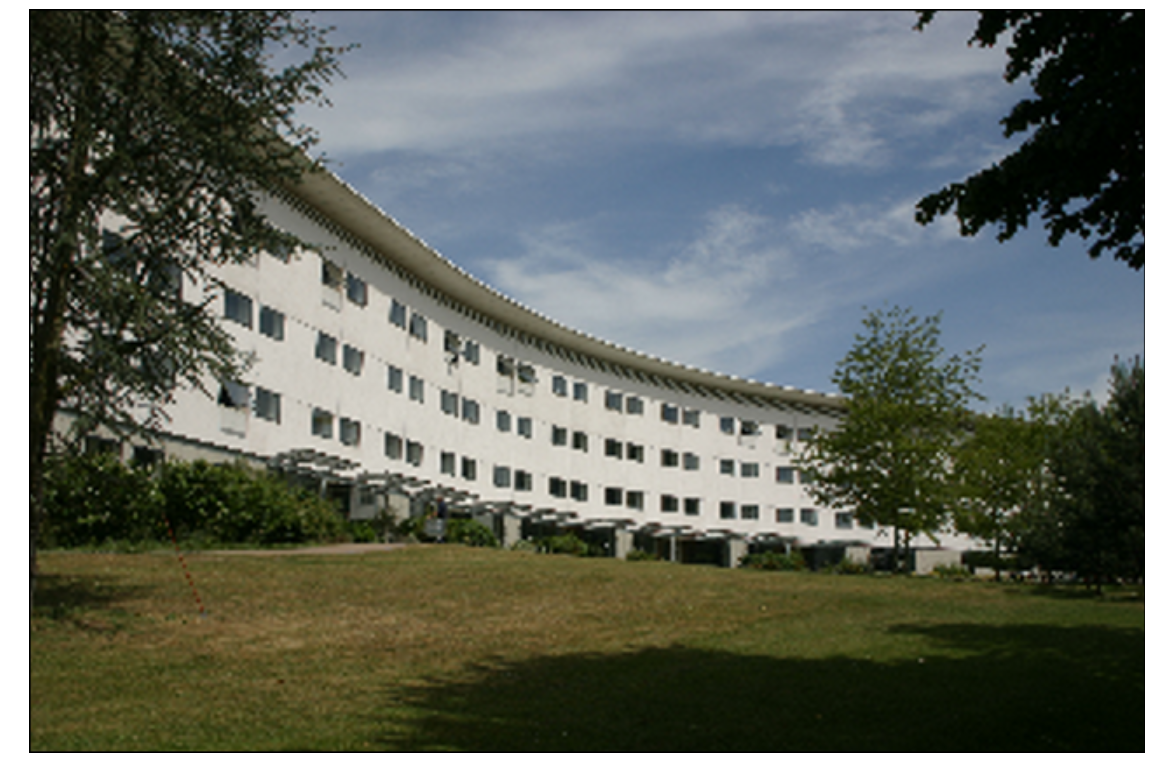
\includegraphics[width=\linewidth]{structured_prediction/images/scene_sp_org}&%
    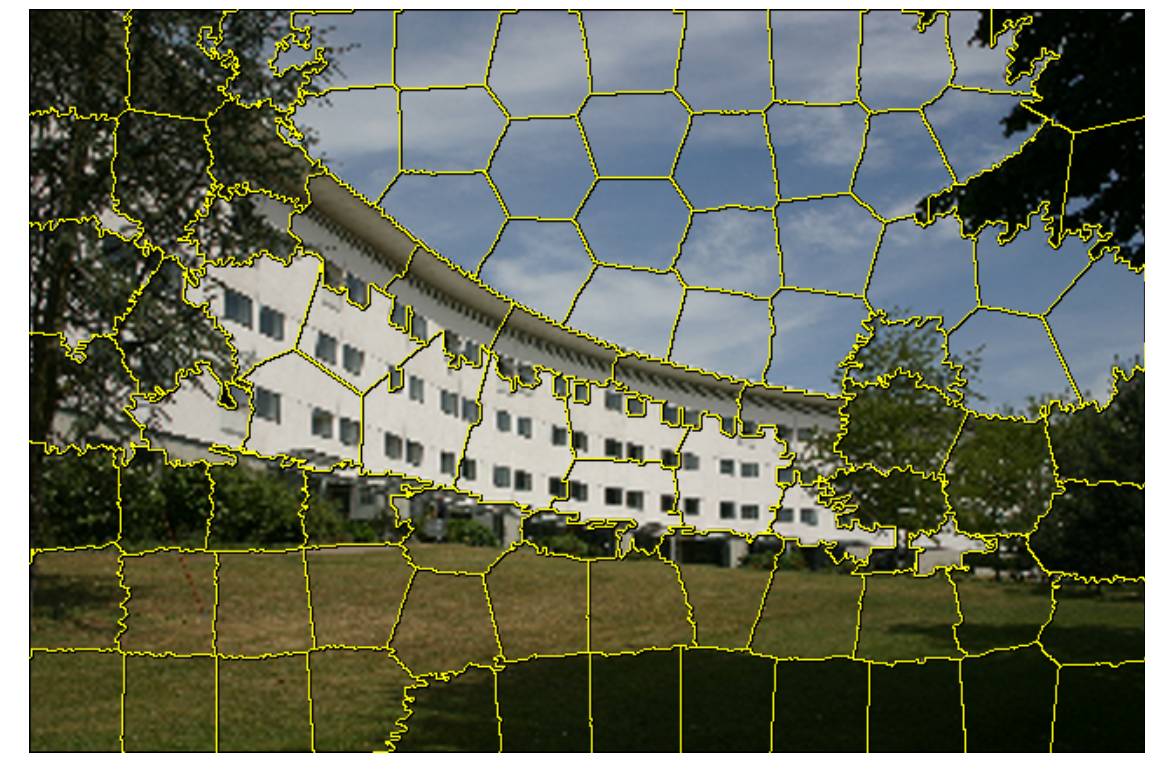
\includegraphics[width=\linewidth]{structured_prediction/images/scene_sp}\\
    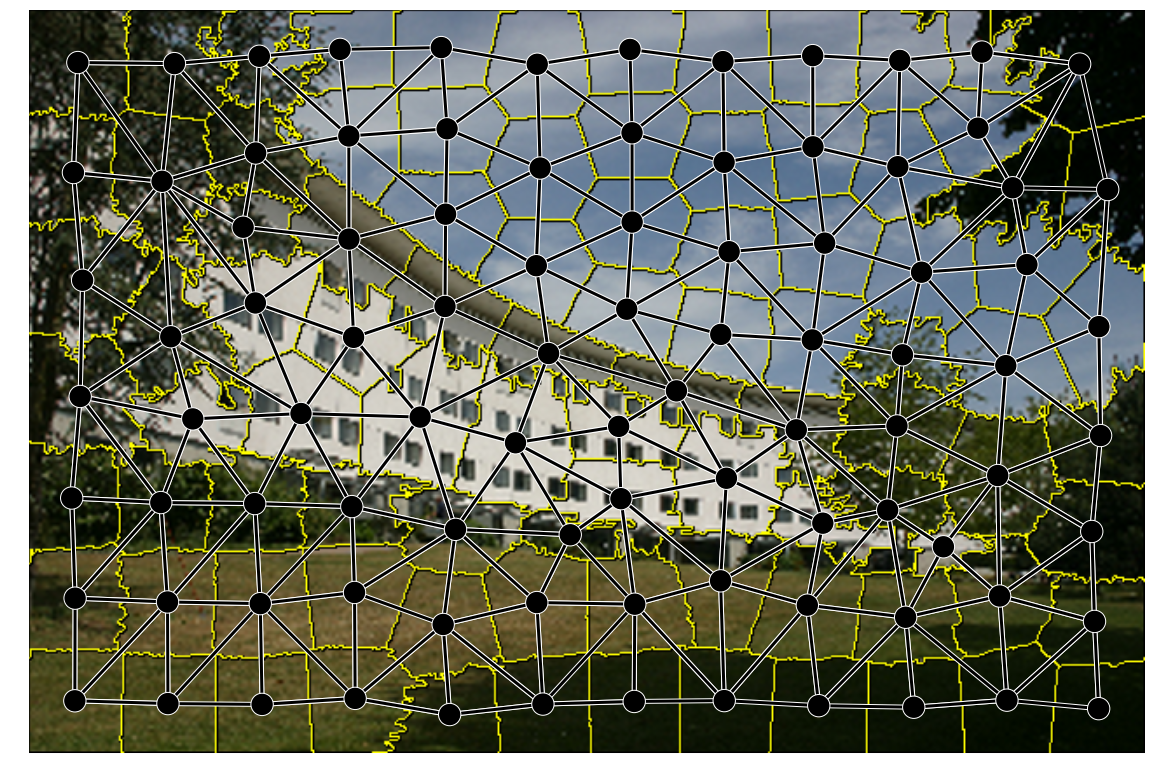
\includegraphics[width=\linewidth]{structured_prediction/images/scene_sp_graph}&%
    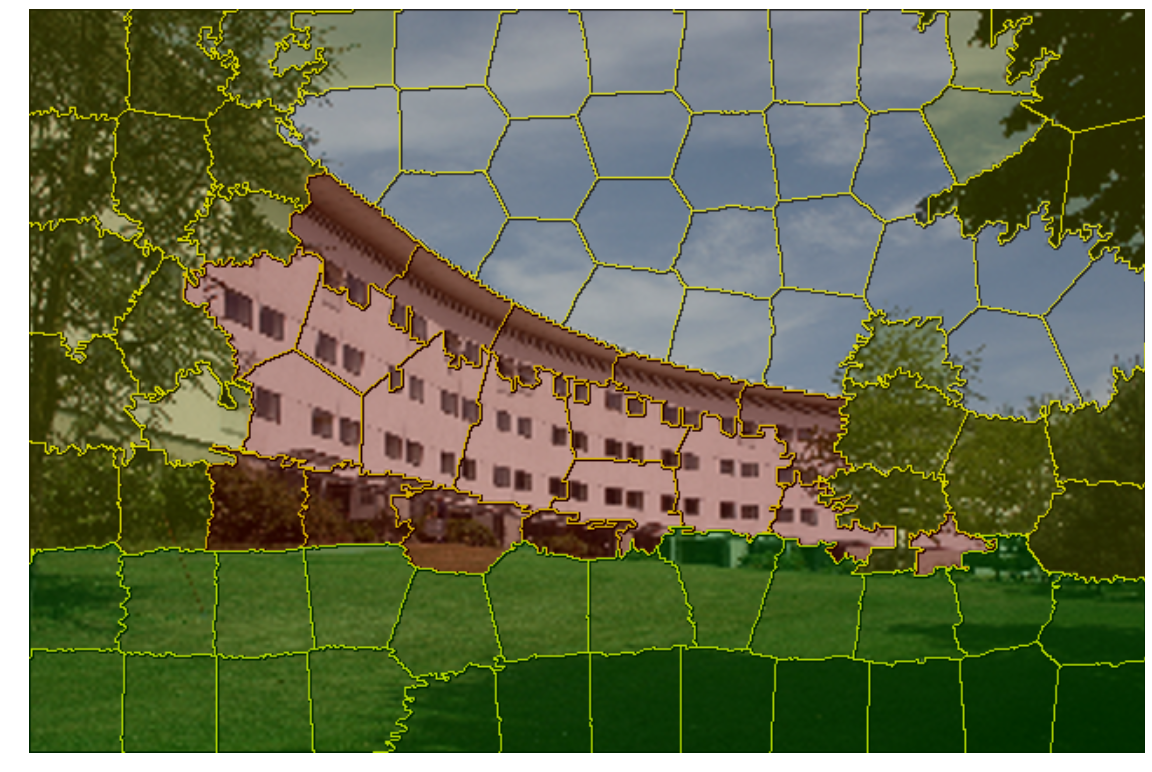
\includegraphics[width=\linewidth]{structured_prediction/images/scene_sp_gt}
\end{tabu}
\caption{%
    Schematic of CRFs over superpixels. From left to right: input image, superpixel segmentation
    using SLIC into about 100 superpixels, pairwise potential in the CRF, and desired labeling.
\figlabel{superpixel_illustration}}
\end{figure}

% hierarchical\dots has superpixels and pixels?

% submodular/non-submodular? higher order?
\subsection{Previous Work}
Conditional random fields were first used in the context of semantic
segmentation by \citet{he2004multiscale}.  Who used contrastive divergence for
learning parameters. Many other early models, such as the one of
\citet{shotton2006textonboost}, did not learn parameters at all, but used
\emph{contrast-sensitive Potts potential}. These potentials have a smoothing
effect over labels by encouraging neighboring variables to take the same value.
The penalty for taking different values is dependent on color contrast between
the pixels.

This smoothing approach was improved upon by \citet{kohli2009robust}, who
introduces higher order potentials to enforce label consistency within larger
regions. Later, \citet{ladicky2009associative} proposed a hierarchical model
over pixels and superpixels, including the higher order potentials of
\citet{kohli2009robust} and additional lateral and hierarchical connections. A
similar approach, using superpixels as the finest resolution, and additionally
modelling object class coocurrences was suggested by
\citet{gonfaus2010harmony}.  However, all these models did not learn the
potentials of the CRF model in a principled manner.  The above approaches all
learned unary potentials using a non-structured approach, for example SVMs or
boosting, and then set pairwise and higher order potentials in the model by
hand.

\citet{szummer2008learning} on the other hand used a structured support vector
machine approach to learn unary and pairwise parameters. They use the classical
graph cut approach of \citet{boykov2001fast} for inference.  However, graph-cut
inference is only applicable to submodular energies, and therefore severely
restricts the expressiveness of the resulting model.
\citet{lucchi2011spatial} investigated the importance of global constraints,
using an approach similar to \citet{szummer2008learning}, but also learning
global interactions---however, these did not improve performance, compared to
simply including global descriptors into local classifiers.

The problem of approximate inference was addressed elegantly by
\citet{yao2012describing}, who learn a joint model for scene classification,
object localization and semantic segmentation.  Their work is based on
\citet{hazan2010primal}, who integrate learning and inference in a joint
optimization problem.

\subsection{Data, Features and Superpixels}
When evaluating learning algorithms in Chapter~\ref{ch:comparison} and
Chapter~\ref{ch:exact_learning} we use the well-established \textsc{Pascal} VOC 2010 and
MSRC-21 datasets, shown in the introduction in \Figref{pascal_msrc}.
As we focus on the learning algorithms in these chapters, we use features for
unary potentials from the literature.

For both datasets we use the TextonBoost class probabilities provided by
\citet{krahenbuhl2012efficient}. For the \textsc{Pascal} VOC dataset, the potentials
provided by \citet{krahenbuhl2012efficient} also include the responses of
object detectors~\citet{}, to better capture the complex object classes.
We average the potentials inside superpixels and use the resulting feature
as input to our unary potentials.
For the MSRC-21 dataset, we compute TextonBoost on two different scales, as
suggested by \citet{mottaghianalyzing}. We additionally extract SIFT and color descriptors and create
bag-of-word descriptors for each superpixel. Following the approach of
\citet{lucchi2011spatial} we augment these with a global bag-of-word descriptor
for each image. We train a linear SVM using an approximation to the additive
$\chi^2$ kernel~\citet{vedaldi2010efficient} and use the response as an
additional input to our CRF\@. This \emph{piecewise training} simplifies
learning and was found to have little effect on
accuracy~\citet{nowozin2010parameter}. In total, there are $63$ features
for the MSRC-21 dataset, $21$ for each scale of TextonBoost and an additional
$21$ for the bag-of-word model using an SVM.

We use the SLIC~\citep{achanta2012slic} algorithm to create superpixel for all
our experiments.  It has been shown to provide competitive results with a
minimum of computational complexity.  Algorithmically, SLIC simply computes a
$k$-means clustering over pixels. Each pixels is represented as 5D point, using
three color channels and the $x$ and $y$ coordinates in the image.  In a
post-processing step, small segments are removed. To make clustering of so many
points feasible, the search for the nearest cluster in $k$-means is restricted
to a local neighborhood in the image. An example of superpixels computed with
the SLIC algorithm can be found in \Figref{superpixel_illustration}.

The features and superpixel algorithm used for the RGB-D dataset NYU used in
Chapter~\ref{ch:nyu} will be discussed there.
